% applogic.tex
\documentclass[dareport.tex]{subfiles}

% Comment it if Build from the main tex i.e. dareport.tex
% Locally usepackage
%
%\usepackage{enumitem}



\begin{document}
% Content here
\section{Application Logic}
The system architecture of the Strike System starts with simple and straight forwards approach. Figure~\ref{fig:strike_arch} shows the basic building block of clients-to-servers and server-to-server processes, and their communication flow.

\begin{figure}[h]
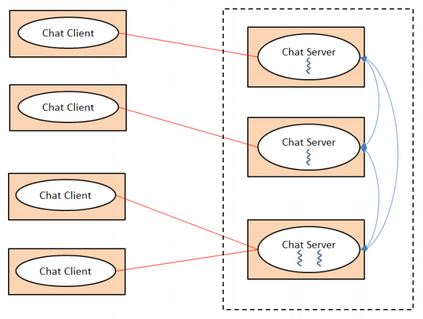
\includegraphics[scale=0.9]{strike_architecture.jpg}
\centering
\caption{Basic Strike Architecture}
\label{fig:strike_arch}
\centering
\end{figure}

\subsection{Requirement Specification}
To begin with, we will discuss the requirement specification and assumption of the application logic. 

\begin{enumerate}[leftmargin=*]
\item Any chat client can connect to any chat server process to perform any of the following operations.

\item A chat client shall authenticate the user using username and password to let the user login to the system. This authenticated session shall maintain until the user logout from the system. The system should also invoke session timeout event to let the user auto-logout from the system if the user has been idle for a specified time. This authenticated session and all chat communication channel shall be encrypted and secured. 

\item An authenticated chat client shall let the user choose their prefer chat nickname (also known as identity or screen-name). After the user selected the nickname, this chat nickname shall be unique throughout the user current logon session. Each chat server must maintain information on this nickname as well as the logon user session and its connected server information. This nickname shall also be globally unique across all server processes i.e. if a user pick a chat nickname "victor" then no other user can create the same chat nickname until the user voluntarily logout or the session timeout has occurred.

\item Each server shall initially create the "MainHall" chat room suffix by server name e.g. if server name is 1 then it will have "MainHall-1" chat room. The logon user shall initially place into this "MainHall" chat room as a default chat room. Each server shall maintain a list of globally available chat rooms i.e. chat rooms from other server as well as chat rooms from locally connected clients. The connected clients shall be able to view this chat rooms list.

\item An authenticated chat client shall allow the user to create the chat room. A chat room will have a name and this chat room will be unique globally i.e. if a user creates a chat room name "joke" then no other user can create another chat room with the same name. Then the user who created the chat room shall become the owner for the chat room. A user can own one chat room at a time. If a client creates a chat room then that chat room will be managed by the server that the client is connected to.

\item An authenticated chat client shall allow the user to delete the chat room that they owned. Only the chat room owner shall be able to delete the chat room. The chat room owner shall delete the chat room first if he/she would like to join another chat room. A chat room is deleted if the owner client quits or disconnects abruptly. If the chat room is deleted, all users inside the chat room shall place into the default chat room i.e. "MainHall" of the connected server.

\item An authenticated chat client shall allow the user to join the chat room. Clients who are members of a chat room must be connected to the server managing that chat room. If a client joins a room managed by the server it is connected to then the server simply places the client in the corresponding room. If the room is managed by another server then the server sends a message to the client redirecting it to the server managing that chat room, without login again.

\item If a chat client disconnects abruptly or quit then the server should handle this and perform a graceful de-registering of the chat nickname and chat room (if owner) from the server. It should also notify this event to its all peer servers and all the peer servers should perform necessary measure to maintain each of their own server state.

\item The chat message must be forwarded to the connected server and, the server should broadcast this chat message to all clients inside the chat room that the user is sending to. The chat server should timestamp the chat message using UTC\footnote{Coordinated Universal Time} before broadcasting back to all the clients. The chat server should synchronize the system time with external NTP\footnote{Network Time Protocol} server in correct timezone.

\item If a chat server crashes or stops responding then other chat servers should detect this situation --- Failure Detection. All chatrooms on that server should be removed from the list and clients should not be redirected to that server anymore until it come back to alive. The connected clients are simply getting disconnected in the case of a chat server crash.

\end{enumerate}

However, this requirement specifications are by no means an exhaustive list but it gives an indication of how the Strike System application logic may behave at this point of implementation. The limitations, assumptions and new features can reiterate and improve as this software project progress along further.

\subsection{Protocol Design}
The core concept of Distributed Systems defines software components 
located at networked computers \textbf{communicate and coordinate their actions only by passing messages}\cite{coulouris}. The protocol specifies exactly how the clients-to-servers and server-to-server communication happen. Therefore, in our Strike System implementation, the protocol design becomes a crucial part of the system. The communication message has to be consistent and serializable. For this we choose JSON\footnote{http://www.json.org/} which is a lightweight data-interchangeable format. The following examples explain the basic building block of how JSON message are passing between client-server and server-server processes.

\begin{enumerate}[leftmargin=*]

\item Example: \textbf{List Server Protocol}
\\
The client can ask for the list of servers in the system and, send to server as a JSON message:
\begin{small}
\begin{verbatim}
{"type":"listserver"}
\end{verbatim}
\end{small}

The server replies with a list of all the servers in the system:
\begin{small}
\begin{verbatim}
{
    "type":"serverlist", "servers": 
    [ 
        {"serverid":"1", "address":"192.168.0.1", "port":"4444"}, 
        {"serverid":"2", "address":"192.168.0.2", "port":"4444"}
    ]
}
\end{verbatim}
\end{small}
In this example, the generated protocols are \verb|type|, \verb|listserver|, \verb|serverlist|, \verb|servers|, \verb|serverid|, \verb|address| and \verb|port|. This is a simple client-server protocol example. We will see a more moderate complex protocol example in next.

\item Example: \textbf{Login Authentication Protocol}
\\
At Login screen, the client send a user authentication message to the server:
\begin{small}
\begin{verbatim}
{"type":"authenticate", "username":"victor", "password":"cheese"}
\end{verbatim}
\end{small}
The chat server will then check the username and password in the user database and attempt to authenticate the user. If the authentication has failed, the server will response to the client with the message:
\begin{small}
\begin{verbatim}
{"type":"authresponse", "success":"false", "reason":"UnknownAccountException"}
\end{verbatim}
\end{small}
The user database can be a centralized database system such as making use of third party database management software. In our implementation, we use Apache Shiro\footnote{https://shiro.apache.org/} framework to make an abstraction for the concrete implementation. As such, the fail reason depends on this middleware specific exceptions. For example, \textit{UnknownAccountException}, \textit{IncorrectCredentialsException}, \textit{LockedAccountException}, \textit{AuthenticationException} are possible Shiro exceptions that can response to the client.
However, if the authentication is success, the chat server response to the client with message:
\begin{small}
\begin{verbatim}
{"type":"authresponse", "success":"true", "reason":"none"}
\end{verbatim}
\end{small}
And, at the same time, the chat server also send to all other servers with message:
\begin{small}
\begin{verbatim}
{
    "type":"notifyusersession", "sessionid":"ba64077b-85b4-40f0-a5ac-480ad3e341b3", 
    "username":"victor", "serverid":"1", "status":"login"
}
\end{verbatim}
\end{small}
When the user logout, the chat server send to all other servers with message:
\begin{small}
\begin{verbatim}
{
    "type":"notifyusersession", "sessionid":"ba64077b-85b4-40f0-a5ac-480ad3e341b3",
    "username":"victor", "serverid":"1", "status":"logout"
}
\end{verbatim}
\end{small}
In this example, the generated new protocols are \verb|authenticate|, \verb|username|, \verb|password|, \verb|authresponse|, \verb|success|, \verb|reason|, \verb|notifyusersession|, \verb|sessionid| and \verb|status|. Note that how it reuse \verb|serverid| protocol keyword from previous example. We use Java Enum\footnote{https://docs.oracle.com/javase/tutorial/java/javaOO/enum.html} type for the protocol keyword definition in Strike Common module package. When implementing a new feature like above example, if there is existing protocol keyword then it will be reused. Otherwise, the new protocol keyword will be created. 
\end{enumerate}

With this approach, the consistent chat protocols are implemented for all the requirement specifications. For the interest of the report length, we will not go through details about every application logic implementation for all the requirement specifications. However, we will still present about details protocol use in follow by sections of our main topics discussion.

Essentially, this JSON based protocol design may yield as \textbf{JMPP} - \textbf{J}SON \textbf{M}essaging and \textbf{P}resence \textbf{P}rotocol, in contrast to XMPP\footnote{https://xmpp.org/} --- in a hope of designing the protocol in more comprehensive and standardize way. In fact, in our initial survey for chat protocol design, we have considered XMPP and IRC protocol specification. However, neither fit to our intention for this project as both specification consider very comprehensive standard to implement, i.e. not light enough for a simple chat system. Furthermore, XMPP is in XML format\cite{xmpp} and IRC is in plain-text format\cite{irc} where we find JSON is more appealing choice for our intention for a simple messaging protocol design.

\subsection{Communication Sub-system}
The another key aspect of the Strike System is the choice for the communication sub-system whereas we consider the chat application protocol (JMPP, so to speak) ride on top of transport layer protocol suite. For this, we choose TCP/IP protocol suite for both client-server and server-server communication. The main reason being is because TCP is a reliable communication protocol whereas --- a stream of data sent on a TCP connection is delivered reliably and in order at the destination\cite{tcp}. The secondary reason being is the SSL/TLS protocol on top of TCP where it satisfies communications security over the Internet and message encryption requirement\cite{tls}. However TCP is unicast communication by design i.e. it requires establishing point-to-point connection and maintaining the TCP stream pipe. 

Since Strike is a chat system, it is by nature a group oriented communication, for example consider chat room and server-to-server communications. Considering for this group communication aspect, Multicast is next appealing choice of communication pattern, especially IP Multicast. IP multicasting is the transmission of an IP datagram to a "host group", a set of zero or more hosts identified by a single IP destination address\cite{ipmcast}. Most common transport layer protocol to use multicast addressing is UDP. UDP is transaction oriented, and it does not guarantee an ordered-reliable-delivery and message duplicate protection\cite{udp}. However, there exist Reliable Multicast algorithms and solutions for ordering of Multicast messages\cite{coulouris}. For researching purpose, our team have attempted implementing Reliable IP Multicast in separate project \textbf{xmcast}. We also survey on popular chat and IM\footnote{Instant Messaging} applications for their use of communication transport layer. Interestingly enough, we find that most IM applications use TCP. 

\begin{enumerate}[leftmargin=*]

\item IRC has been implemented on top of TCP --- \cite{irc} section \emph{8.1 Network protocol: TCP}.

\item XMPP use of TCP is quite visible --- \cite{xmpp} sections \emph{2.3.Persistent Streams} and \emph{3.TCP Binding}. Some popular implementation of XMPP includes Apple Mac iChat Server, Google Talk(early version), Facebook Messenger(early version), WhatsApp.

\item In 2012, WhatsApp has announced 2 million TCP connections which retrospective to 1 million TCP connections in 2011\cite{whatsapp}.

\end{enumerate}

Base on this survey as well as where we like to focus on developing a simple functioning chat application, our team has prioritized on building Strike communication sub-system to be on top of TCP. However, IP Multicast with our own \textbf{xmcast} module implementation or JGroups\footnote{http://jgroups.org/} is still viable alternative solution for Strike System, especially if we consider offering video and voice chat feature as this software project progress along further.

\subsection{Multi-threading, Concurrency and ServerState}
In socket programming, it is inevitable that the incoming steam readings are blocking calls. It is essential to program the socket communication with multi-threads programming. Strike chat server is primarily responsible for managing all the clients concurrently connected to it and for broadcasting chat messages. For this purpose, TCP connections between clients and servers are established and remain active throughout the duration of the client-server interaction. It is also the responsibility of the server to maintain the consistent \textbf{ServerState} of the connected TCP client and associated thread(s), the user's chat nickname, the chat room created by the user. The server has to synchronize these states after sending the appropriate protocol message to the client. For server-to-server communication, the TCP connection can be a short-live connection i.e. open and close as each message send or receive. 

In our approach to multi-threading, we make use of Java Thread Pools\footnote{https://docs.oracle.com/javase/tutorial/essential/concurrency/pools.html} feature. When the \textbf{StrikeServer} is bootstrapping, the entry main method create two threads from its service pools namely \textbf{ClientService} and \textbf{ManagementService}. These services manage server socket and accepting the incoming connections on client port and management port respectively. We will go through \textbf{ClientService} for example below.

\begin{enumerate}[leftmargin=*]

\item In \textbf{ClientService}, when message arrive at server socket, it creates \textbf{ClientConnection} with the accepted client socket.

\item The \textbf{ClientConnection} creates the single thread pool for \textbf{MessageReader} with referencing to its client socket input stream reader and message \textbf{BlockingQueue}.

\item As the message arrive, it will take the message from message queue and delegate to protocol handler to handle the message.

\item \textbf{ProtocolHandlerFactory} will then create appropriate client handler based on incoming message protocol type. These concrete protocol handlers implement \textbf{IProtocolHandler} interface handle method as shown in Figure~\ref{fig:protohdl}. Additionally it will also update \textbf{ServerState} as if required.

\end{enumerate}

\begin{figure}[h]
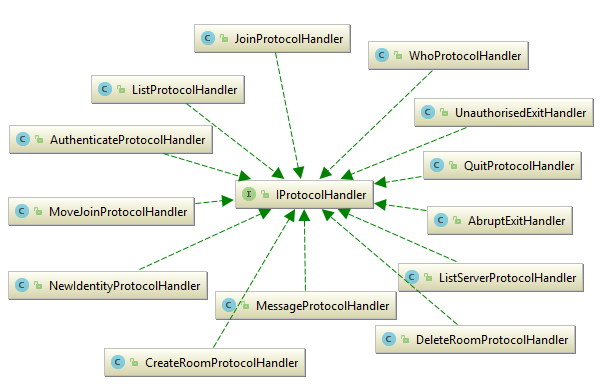
\includegraphics[scale=0.9]{strike_protocol_handlers.png}
\centering
\caption{Strike Server - Protocol Handlers}
\label{fig:protohdl}
\centering
\end{figure}

Figure~\ref{fig:clientsq} shows the sequence diagram about how these classes orchestrate to run concurrently to handle incoming and outgoing client messages. Similarly, the \textbf{ManagementService} and \textbf{ManagementConnection} is implemented in the same concurrent approach for server-to-server communications. Protocols handling are implemented in Factory creation design pattern to be defensive programming for concurrency proof --- i.e. these handler objects will be cheaply created and garbage collected efficiently.

\begin{figure}[h]
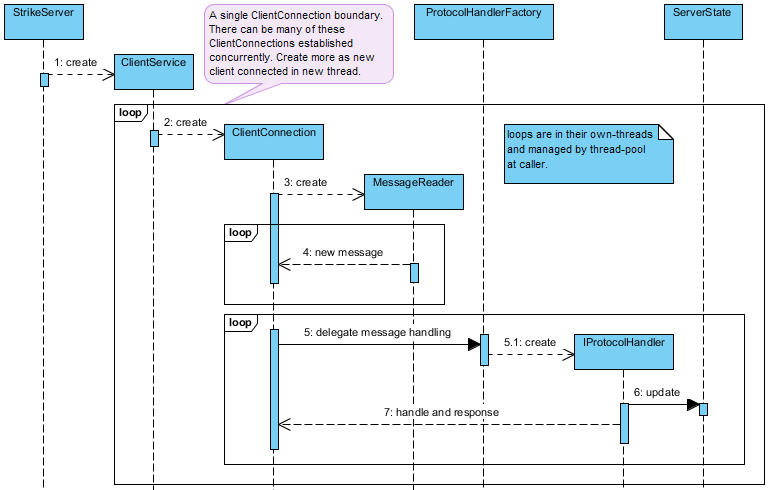
\includegraphics[scale=0.9]{strike_server_client_conn.png}
\caption{Strike Server - Client Connection Sequence Diagram}
\label{fig:clientsq}
\centering
\end{figure}

\textbf{ServerState} object is the critical region of the Strike server where it stores the state of the server in memory. It is an Singleton object and there is only single existence throughout the application life cycle. Its data structure properties are backed by Java Concurrency data structure as well as use of Java \textbf{synchronized} keyword on non-concurrency data type. The \textbf{ServerState} properties can be easily persisted into persistent store such as Database Management System as this software project progress along further.

\end{document}